% Farbkarte TU Darmstadt: http://www.webteam.tu-darmstadt.de/media/webteam_wissensdatenbank/artikel_1/farbkarte_TU_Darmstadt.png
\documentclass[nochapterpage,nopartpage,noheadingspace,numbersubsubsec,bigchapter,colorback,accentcolor=tud9c,10pt]{tudreport}
\usepackage[ngerman,english]{babel}

\usepackage[stable]{footmisc}
\usepackage[ngerman,english]{hyperref}

\usepackage{longtable}
\usepackage{multirow}
\usepackage{booktabs}

% Custom packages
\usepackage{wrapfig}
\usepackage{etoolbox}
\usepackage{multicol}
\usepackage{listings}

\lstset{
    breaklines=true,
    postbreak=\raisebox{0ex}[0ex][0ex]{\ensuremath{\color{red}\hookrightarrow\space}}
}

% Reset chapter counter after introducing a new part and start chapters on the same page
\makeatletter
\@addtoreset{chapter}{part}
\patchcmd{\scr@startchapter}{\if@openright\cleardoublepage\else\clearpage\fi}{}{}{}
\makeatother

\hypersetup{%
  pdftitle={Internet Praktikum TK Documentation},
  pdfauthor={M. Schanz},
  pdfsubject={Project Documentation},
  pdfview=FitH,
  pdfstartview=FitV
}

%%% Zum Tester der Marginalien %%%
  \newif\ifTUDmargin\TUDmarginfalse
  %%% Wird der Folgende Zeile einkommentiert,
  %%% werden Marginalien gesetzt.
  % \TUDmargintrue
  \ifTUDmargin\makeatletter
    \TUD@setmarginpar{2}
  \makeatother\fi
%%% ENDE: Zum Tester der Marginalien %%%

\newlength{\longtablewidth}
\setlength{\longtablewidth}{0.7\linewidth}
\addtolength{\longtablewidth}{-\marginparsep}
\addtolength{\longtablewidth}{-\marginparwidth}

\title{Internet Praktikum TK 2016\\ Conference Management System\\ Team Whisky}
\subtitle{Auel, Tarek,\\ Sahin, Huzeyfe\\ Schanz, Markus}


\begin{document}
\maketitle
\tableofcontents
%\listoffigures
%\addcontentsline{toc}{chapter}{\listfigurename}



\part{Technical Documentation}
\label{part:tech}

  \chapter{Introduction}
  \label{ch:tech:intro}

    This part of the documentation is intended for server administrators and/or developers who want to setup the project on their local machine. The documentation is written such that the individual chapters can be read in arbitrary order. Each chapter is a self-contained piece of documentation. However, the software tools listed in the following section~(\ref{sec:tech:3rd-party}) are heavily used throughout the application. Therefore, a short introduction to them is given in this chapter. For further information please refer to the individual project sites. Appendix~\hyperref[ch:appendix:setup]{A} hold the instructions on how to setup the application on a local machine.

  \section{Third Party Software}
  \label{sec:tech:3rd-party}

    The application utilizes third party software \& libraries in order to keep the codebase clean and allow for a productive development. This section gives an overview of the most important third party libraries \& tools that the project relies on.

  \paragraph{Node.js \& Node Package Manager}
    This project uses \emph{Node.js} as a runtime environment on the server.%
    \footnote{\url{https://nodejs.org/}}
    In recent years, \emph{Node.js} became very popular as it allows the developer to use JavaScript for both server and client programming. It comes bundled together with its own package manager \emph{npm} which can be used to install a wide variety of third party libraries that further ease the development process.

  \paragraph{StrongLoop}
    \emph{StrongLoop} is a mandatory library on which the application is primarily build upon.%
    \footnote{\url{https://strongloop.com/}}
    This tool is able to generate code files for both server and client that can be used to manipulate a previously defined database schema. It can be installed (and kept up-to-date) via \emph{npm}.

  \paragraph{Bower}
    Analogous to \emph{npm}, \emph{Bower} is a package manager for JavaScript libraries.%
    \footnote{\url{https://bower.io/}}
    However, \emph{npm} manages libraries that are required for the server part of the application (Node.js) whereas \emph{Bower} focuses on the management of libraries that are used on the client side, i.e., in the browser.

  \paragraph{AngularJS}
    AngularJS is a web application framework that is utilized by the application.%
    \footnote{\url{https://angularjs.org/}}
    It eases development by providing a model-view-controller (MVC) like architecture. The code that is generated by \emph{StrongLoop} is also targeting the AngularJS framework.\\


    The remainder of this documentation is structured as follows: Chapter~\ref{ch:tech:architecture} gives an insight of how the application works conceptually. It covers the directory structure of the project as well as basic concepts and important files that are involved in bootstrapping the application. Implementation details such as authentication, authorization, etc. are covered in chapter~\ref{ch:tech:implementation}. Eventually, chapter~\ref{ch:tech:handson} describes the process of extending the application, i.e., how to extend the navigation, add a new page, etc.

  \chapter{Architecture}
  \label{ch:tech:architecture}

        \begin{figure}
            \centering
            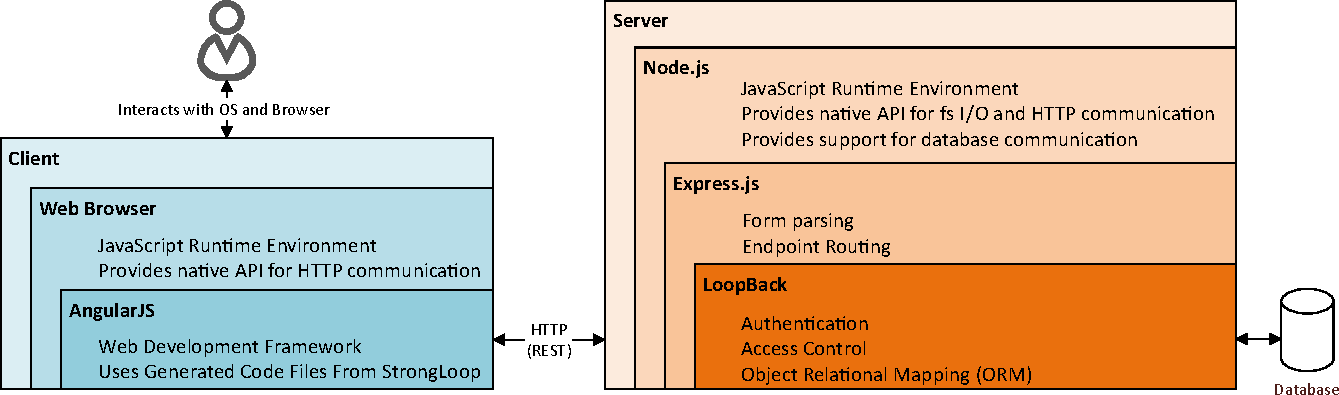
\includegraphics[width=\textwidth]{architecture-horizontal}
            \caption{Architecture.}
            \label{fig:architecture}
        \end{figure}

        %\begin{wrapfigure}{r}{0.5\textwidth}
        %\begin{figure}
        %    \centering
        %    \includegraphics[width=0.48\textwidth]{TUDreport-fig}
        %    \caption{In curley braces.}
        %    \label{fig:client-server}
        %\end{figure}
        %\end{wrapfigure}
    On a high-level view, the application follows a client-server approach. The server part of the application primarily manages the database and provides a public REST API%
    \footnote{\url{https://en.wikipedia.org/wiki/Representational_state_transfer}}
    whereas the client part runs in the browser of the user and provides an user interface (UI). The client part is responsible to translates user interactions into requests against the server API and reflect the responses in the UI. %Figure~\ref{fig:client-server} illustrates the above described scenario.

  \section{Project Directory Structure}
  \label{sec:tech:architecture:dirs}

    The top level directory of the project is organized as follows:
        \begin{multicols}{4}

            \begin{itemize}
                \item /bin
                \item /client
                \item /common

                \item /doc
                \item /node\_modules
                \item /server

                \item /storage
            \end{itemize}
        \end{multicols}

    \paragraph{/}
    Besides the listed directories above, the root directory \emph{/} does also contain several files worth mentioning. \emph{bower.json} and \emph{.bowerrc} are the configuration files that are automatically found and loaded by \emph{Bower}. They contain the list of dependencies and version constraints that to be installed by bower. By renaming the database file \emph{db.json.default} to \emph{db.json}, the application can be tested with some predefined seed data.

    \paragraph{/bin}
    Contains executable scripts that are used to initialize the application database with dummy data.

    \paragraph{/client}
    Resembles the root directory that is publicly accessible through the HTTP web server, i.e., it contains all the code that is relevant for the client application.

    \paragraph{/common}
    Holds the models that describe the application database schema. These models are taken into account by \emph{StrongLoop} when generating the client and server code files. The files inside this directory can either be edited manually (according to the format description) or through the \emph{StrongLoop} console line interface.

    \paragraph{/doc}
    Contains all documentation relevant files such as the documentation at hand.

    \paragraph{/node\_modules}
    This is where \emph{npm} stores the depended modules. Besides a \emph{.gitignore} file, this directory is empty when the repository is checked out cleanly.

    \paragraph{/server}
    Contains the code that is executed inside the Node.js environment on the server side. It provides the logic to manipulate data, handles authentication and access control and also provides the public REST API.

    \paragraph{/storage}
    \emph{LoopBack}\footnote{The framework provided by \emph{StrongLoop}} manages file uploads in so-called containers. This directory contains one directory for each container and each of these hold in turn a list of files that were uploaded to the corresponding container. This directory is initially empty when the repository is checked out cleanly. It gets filled once the conference users start to submit their papers.

  \chapter{Implementation}
  \label{ch:tech:implementation}

    Implementation details...

  \chapter{Hands On: Implementation of an Application Section}
  \label{ch:tech:handson}

    What are the required files, how are they included, etc etc.



\part{User Documentation}
\label{part:user}

  \chapter{Introduction}
  \label{ch:user:intro}

    A conference management system...

  \chapter{Attendee}
  \chapter{Author}
  \chapter{Reviewer}
  \chapter{Chair}



\part{Appendix}
\label{part:appendix}

  \chapter*{A.\quad Application Installation}
  \addcontentsline{toc}{chapter}{A.\quad Application Installation}
  \label{ch:appendix:setup}

    The application does not enforce the usage of a specific operating system. However, we recommend to use a Linux system with a package manager in order to install the required prerequisites to make the setup process as smooth as possible.

  \section*{Prerequisites}
  \label{sec:appendix:setup:prerequisites}

    Before starting with the installation process, please make sure that your system does met the following prerequisites:
        \begin{multicols}{2}
        \begin{itemize}
            \item Git $\ge$ 2.x
            \item Node.js $\ge$ 4.2.x
            \item npm $\ge$ 3.x (part of Node.js)
        \end{itemize}
        \end{multicols}

    \noindent The project heavily relies on strongloop for generating API code as well as on bower to fetch 3rd party java-script libraries. To install both on your system execute the following command:
        \begin{lstlisting}[language=bash]
    # npm install -g strongloop bower
        \end{lstlisting}

  \section*{Installation}
  \label{sec:appendix:setup:install}

    \noindent Use the git command to fetch a copy of the source code repository.%
    \footnote{Requires read access to the repository.}
    The command should be executed by the user who is supposed to run the application and inside an empty directory which is going to hold the application source code.
        \begin{lstlisting}[language=bash]
    $ git clone ssh://git@scm.informatik.tu-darmstadt.de/iptk-ss2016/iptk-ss2016-team-whiskey.git .
        \end{lstlisting}
    For further installation instructions, please stick to the \emph{readme.md} file which is now found inside the directory.


  \chapter*{B.\quad Database Entity Relationship Model}
  \addcontentsline{toc}{chapter}{B.\quad Database Entity Relationship Model}

    % Figure of ERM goes here

  \chapter*{C.\quad Application Screenshots}
  \addcontentsline{toc}{chapter}{C.\quad Application Screenshots}

    % Figure of ERM goes here

  \chapter*{D.\quad (Un)Implemented Features}
  \addcontentsline{toc}{chapter}{D.\quad (Un)Implemented Features}

    % List of features goes here
    Below is the list of (un)implemented features, copied from the SCM wiki page.%
    \footnote{\url{https://scm.informatik.tu-darmstadt.de/projects/iptk-ss2016/wiki/Conference_management_system_-_Features}}
    A checked box ($\boxtimes$) means that the feature is implemented whereas an unchecked box ($\square$) means that the feature is (partly) unimplemented
        \begin{itemize}
            \setlength\itemsep{0em}
            \item Roles
            \begin{itemize}
                \item[$\boxtimes$] Authors [0..*]
                \item[$\boxtimes$] Reviewers [0..*]
                \item[$\boxtimes$] Chair [1..*]
            \end{itemize}

            \item General
            \begin{itemize}
                \item[$\boxtimes$] responsive design: access the web application with different kinds of devices (mobile, tablet, pc..)
            \end{itemize}

            \item As a user, I can
            \begin{itemize}
                \item[$\boxtimes$] register to the system at least with email, password
                \begin{itemize}
                    \item[$\boxtimes$] emails are unique
                    \item[$\boxtimes$] users can have multiple roles (e.g., author and reviewer)
                    \item[$\boxtimes$] additional information (see slides)
                    \begin{itemize}
                        \item[$\boxtimes$] e.g., basic profile (given name, family name, postal address)
                        \item[$\boxtimes$] e.g., affiliation (institution, city, state, country)
                    \end{itemize}
                \end{itemize}
                \item[$\boxtimes$] login to the system at least with registered email, password
                \item[$\boxtimes$] edit my profile (password, additional information)
                \item[$\boxtimes$] remove my profile
                \item[$\boxtimes$] logout
            \end{itemize}

            \item As a author, I can
            \begin{itemize}
                \item[$\boxtimes$] create a new submission (if submission is open)
                \begin{itemize}
                    \item[$\boxtimes$] title
                    \item[$\boxtimes$] registered authors [1..*] (given name, family name, email affiliation)
                    \item[$\boxtimes$] abstract
                    \item[$\boxtimes$] keywords (multi-selection) that describe the submission (e.g., research fields)
                    \item[$\boxtimes$] upload the paper (.pdf)
                \end{itemize}
                \item[$\boxtimes$] access current submissions (overview)
                \begin{itemize}
                    \item[$\square$] status: incompleted, completed, closed, accepted, rejected
                \end{itemize}
                \item[$\boxtimes$] look at a submission
                \item[$\boxtimes$] edit a submission (if submission is open)
                \item[$\boxtimes$] withdraw a submission
            \end{itemize}

            \item As a reviewer, I can
            \begin{itemize}
                \item[$\boxtimes$] access assigned submissions (overview + status)
                \item[$\boxtimes$] look at an assigned submission
                \begin{itemize}
                    \item[$\boxtimes$] details, pdf download or view
                \end{itemize}
                \item[$\boxtimes$] make a review > template (if review is open)
                \begin{itemize}
                    \item[$\boxtimes$] reviewer expertise: (1) not familar w/ the topic - (5) expert
                    \item[$\boxtimes$] overall evaluation: (1) strong reject - (5) strong accept
                    \item[$\boxtimes$] summary
                    \item[$\boxtimes$] major strong popints
                    \item[$\boxtimes$] major weak points
                    \item[$\boxtimes$] detailed comments
                \end{itemize}
                \item[$\boxtimes$] edit a review (if reviewing phase is open)
            \end{itemize}

            \item As a chair, I can
            \begin{itemize}
                \item[$\boxtimes$] list all paper submissions
                \begin{itemize}
                    \item[$\boxtimes$] look at a submissions (details, pdf download or view)
                    \item[$\square$] withdraw a submission
                \end{itemize}
                \item[$\boxtimes$] list all authors
                \begin{itemize}
                    \item[$\boxtimes$] look at detail information
                \end{itemize}
                \item[$\boxtimes$] list all reviewers
                \begin{itemize}
                    \item[$\boxtimes$] look at detail information
                \end{itemize}
                \item[$\boxtimes$] list all reviews
                \begin{itemize}
                    \item[$\boxtimes$] look at a review
                \end{itemize}
                \item[$\boxtimes$] assign papers to reviewers
                \begin{itemize}
                    \item[$\boxtimes$] conflict avoidance: an author is not allow to review his own paper
                \end{itemize}
                \item[$\boxtimes$] do the schedule management
                \begin{itemize}
                    \item[$\boxtimes$] automatic: set close deadlines for submissions and reviews
                    \item[$\boxtimes$] manual: (re-)open/close submissions and reviews
                \end{itemize}
                \item[$\square$] view fancy summary charts or reports (e.g., total submission, acceptances, topics, countries etc.)
            \end{itemize}

            \item Bonus features (OPTIONAL)
            \begin{itemize}
                \item[$\square$] users must confirm their registration by clicking on a registration link sent via email
                \item[$\square$] email notification to submitters and reviewers (status changes)
                \item[$\square$] chat with other online authors
                \item[$\square$] automatic assignment (even distribution) and conflict resolving
                \item[$\boxtimes$] a user can create multiple conference events and becomes the chair (=administrator) of them
            \end{itemize}
        \end{itemize}

\end{document}
